\chapter{Motivation}

A water surface wave simulator can provide several advantages when implemented in a flight simulator. This \levelname will take up two of the main reasons for why \Saab wants to implement a wave simulator in their flight.

\HRule

Besides, as an aircraft carrier travels travels with full speed against the wind in order to give the pilot who is supposed to land on it the minimal speed relative to the carrier during the landing, it leaves a wake behind of itself which serves as an aid for the pilot when trying to find the right angle to approach the ship with. Therefore, ships also have to give rise to waves as they travel on the water, which should propagate in a realistic way in order to form the characteristic \idxs{Kelvin}{wake pattern}. Ships should also draw air down into the water in order to give rise to the also so characteristic \backwash that follows like a tail behind a large ship.

It is therefore necessary to in a realistic way simulate waves on the surface of the water, with a two-way interaction between water and ships. This should happen in realtime in order to make it possible to implement it in a \idxs{flight}{simulator}. Simulation of water waves faces a number of challenges, like \idxs{wave}{dispersion}, which makes waves with different \wavelengths travel with different speeds,

the ships have to be able to become affected by surface waves and rock forth and back 

\HRule

\section{Landing on ships with helicopters}

In order for a pilot to get the most out of training in a flight simulator, the pilot has to face similar challenges as in a real world scenario. For some helicopter missions, offshore landings on a ship have to be preformed. The landings are sometimes performed so far offshore that the pilot passes the limit where the fuel that's left in the fuel tank is just enough to return to solid ground. This limit is referred to as \idxs{bingo}{fuel}. If a helicopter that is supposed to land on a ship passes this limit, the only remaining option is to land on the ship.

However, when the ship is small, such as those seen in \citep{MrOawal2009,PrismDefence2010,KopulaDK2010}, and is exposed to large waves, landing on it becomes difficult, as can be seen in \citep{PrismDefence2010}, and if the pilot isn't familiar with landing under such circumstances, it could lead to disaster. It is therefore of high importance that the pilots can train landing on ships under similar circumstances in a simulator, before landing with a helicopter on a rolling ship in a real situation. Hence, it is important that ships in the simulation are affected by waves, in order to get a situiation that is realistic enough to give an good \idxs{training}{value}.

\section{Visual cueing}

In order for the \idxs{human}{perception} to work, and for the \brain to be able to estimate properties in the environment, such as distances, speeds, etc. the brain uses a number of clues it gets from processesing and interpreting \idxs{sensory}{information} by comparing them with earlier processed sensory information from similar experienced situations. These clues are something refered to as \idxsp{sensory}{cue}{s}.

\subsection{Surface disturbances caused by the wind flow from the rotor blades}

When a helicopter pilot flies over a field of grass, he can for example look at how much the grass bends due to the air flow from the rotor blades in order to estimate the distance to the ground. The level of bending of the grass is therefore a visual cue to the brain when it comes to determinig this distance.

Similarly, when a helicopter pilot flies over a body of water on a day with little wind, he can estimate the distance to the surface by looking at surface disturbances, also cause by the air flow from the rotor blades. The level of disturbances on the surface is therefore another visual clue.

\subsection{Wind waves}

On a day with much wind however, it might be difficult to see really how large the surface disturbances caused by the air flow from the rotor blades are, since they are dominated by the waves caused by the wind. On the other hand, those waves also acts as visual cues. First, the more the wind blows, the larger the waves will be and the more likely it is that white foam will form on the crests

\subsection{Landing on ships with aircrafts}

A fighter aircraft that is about to land on an aircraft carrier has to approach the carrier from behind and often slightly from the side, so the pilot has to know the orientation of the carrier. During landing, the carrier traveles with as high speed as possible against the wind in order to give the polit as high relative speed to the air as possible, creating \wake behind itself, with a \backwash that can usually be seen clearly by the pilot. This backwash can be seen in \figref{fig:aircraft_carriers_and_backwash}. In \figref{fig:aircraft_carrier_full_wake}, \idxsp{V-shaped}{wavefront}{s} after the ship can also be observed; these wavefronts form two \idxsp{wake}{line}{s}, one on each side of the backwash, which together are known as the \idxs{Kelvin}{wake pattern}\index{pattern!wake|see{Kelvin wake pattern}} after the British scientist \idxs{Lord}{Kelvin}.

\begin{figure}
    \centering
    \subcaptionbox{\label{fig:aircraft_carrier_full_wake}} {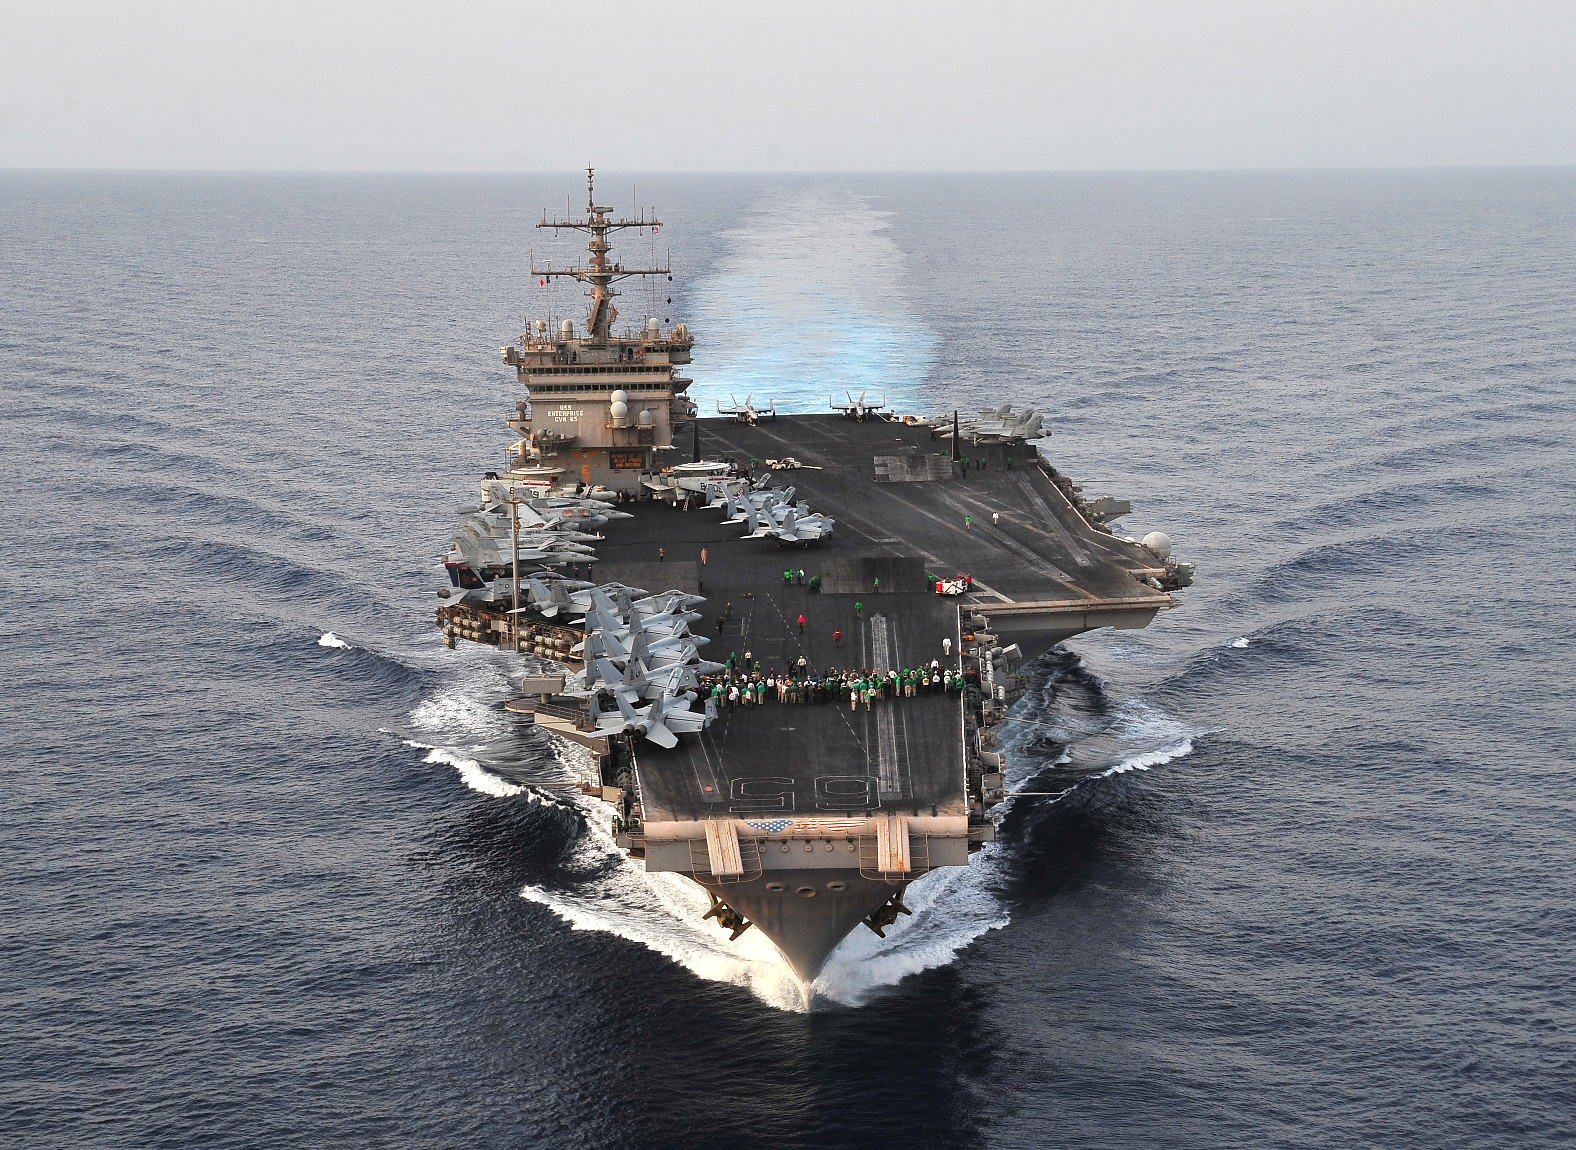
\includegraphics[width=0.495\textwidth]{Images/Public_domain/The_aircraft_carrier_USS_Enterprise_(CVN_65)}}
    \subcaptionbox{\label{fig:aircraft_carrier_landing_backwash}} {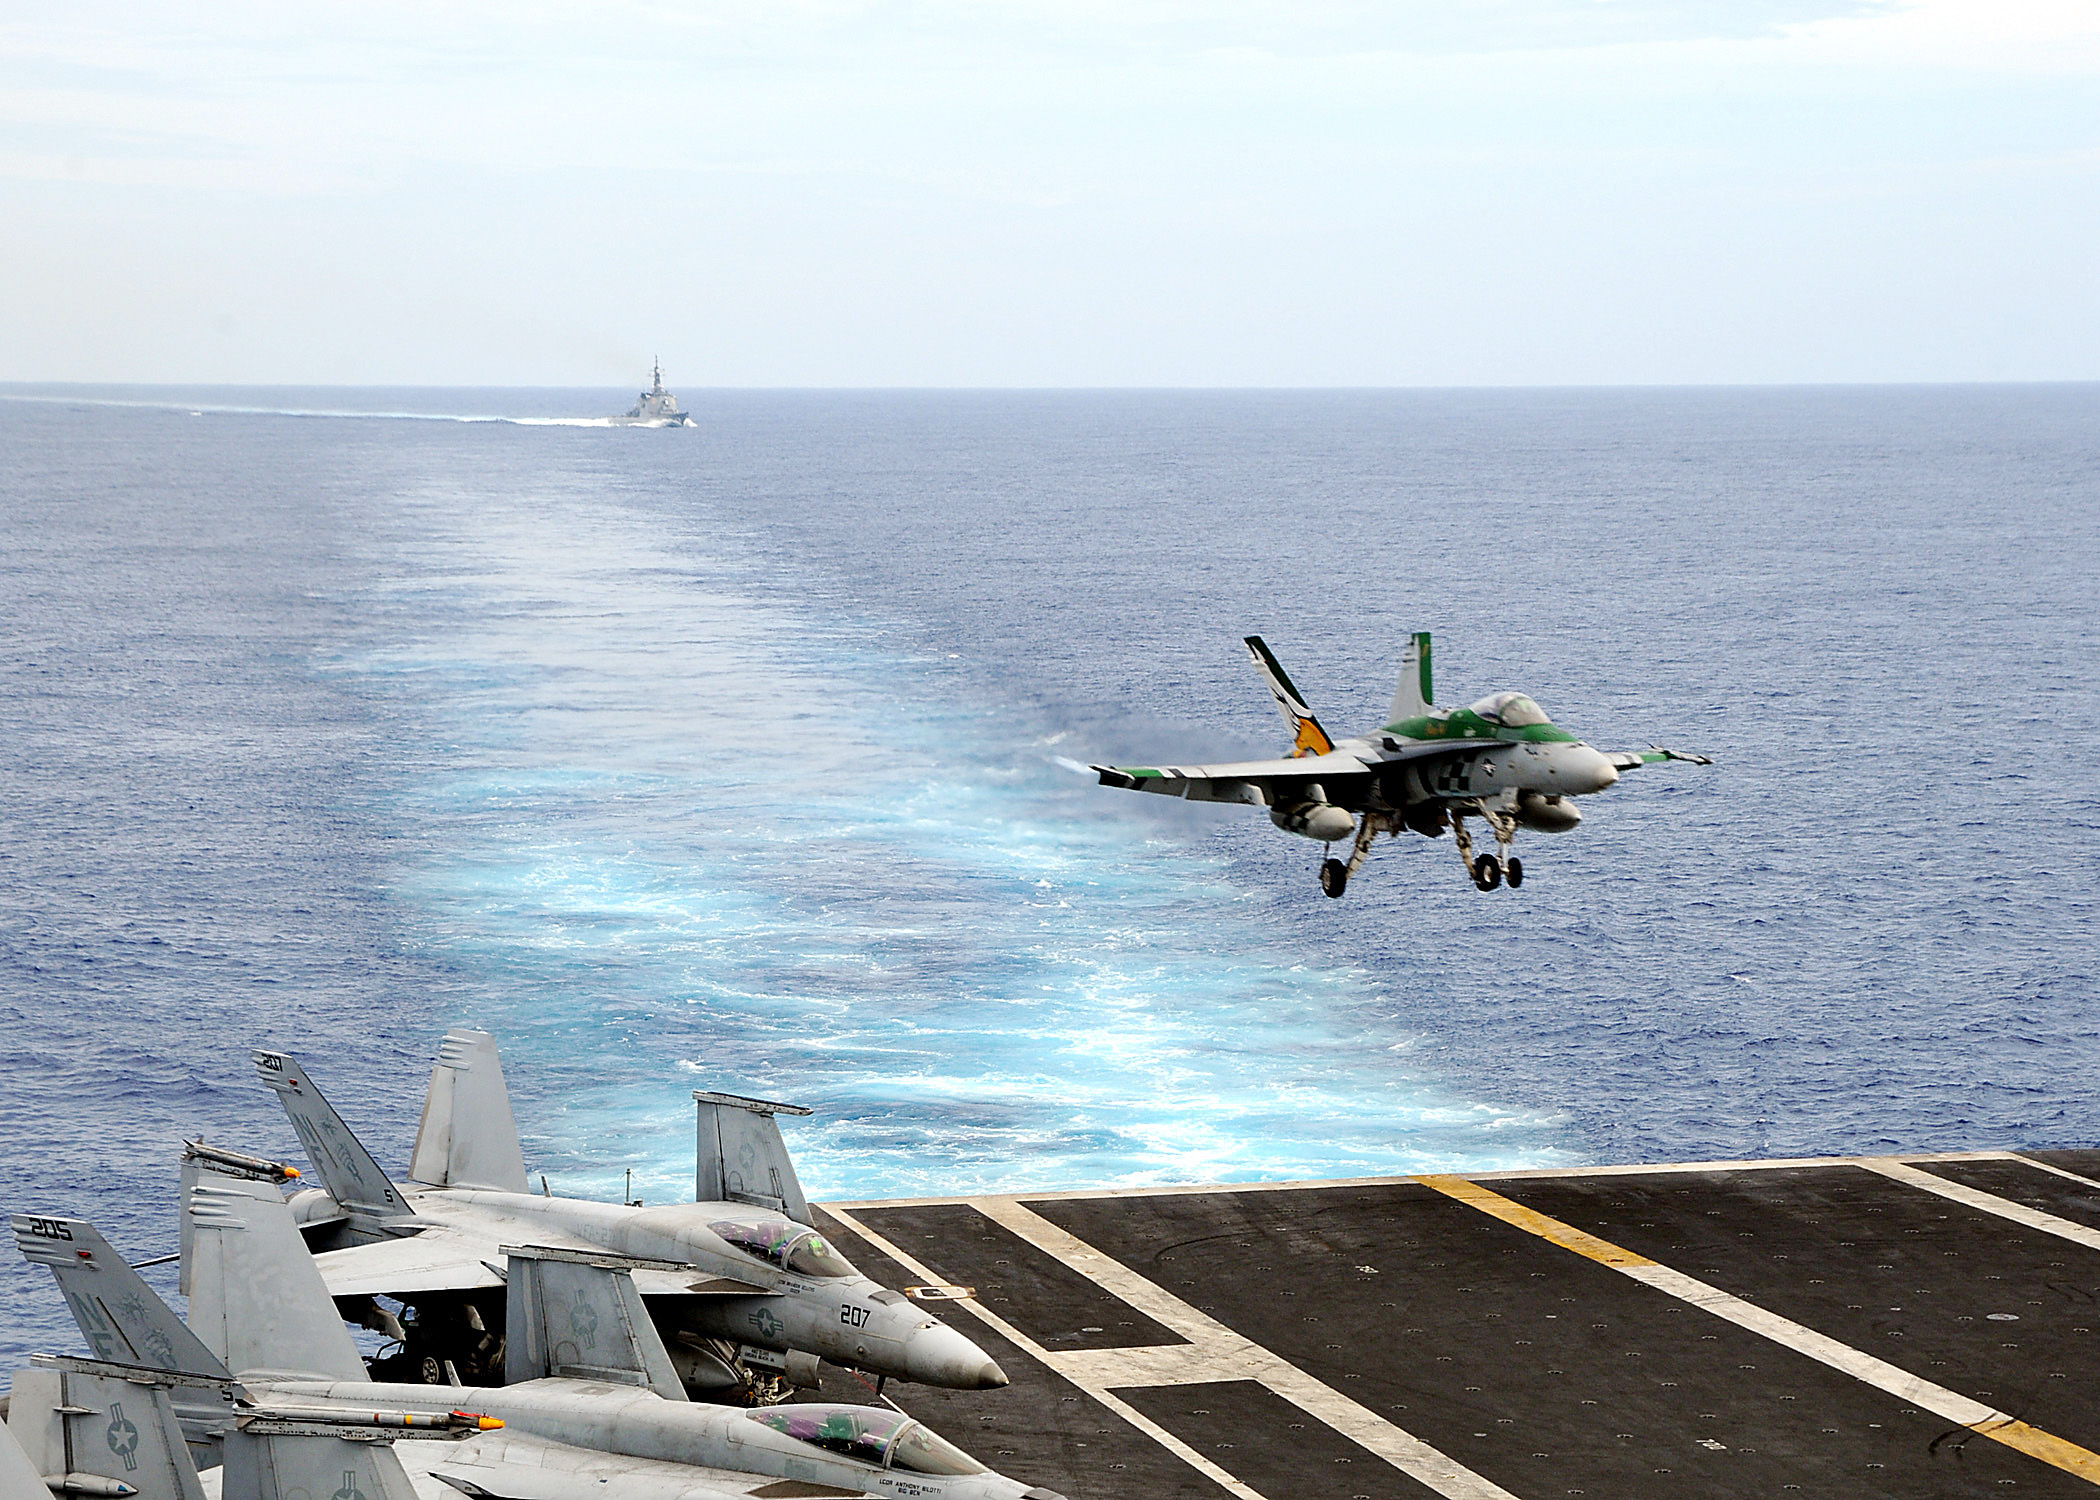
\includegraphics[width=0.495\textwidth]{Images/Public_domain/An_F-A-18C_Hornet_lands_on_the_aircraft_carrier_USS_George_Washington_(CVN_73)}}
    \caption{Aircraft carriers. Note the backwash created behind the ships, serving as a reference for aircraft pilots during landing. \subrefp{fig:aircraft_carrier_full_wake} The aircraft carrier USS Enterprise (CVN 65). \subrefp{fig:aircraft_carrier_landing_backwash} An F/A-18 Hornet landing on an aircraft carrier.}
    \label{fig:aircraft_carriers_and_backwash}
\end{figure}

In a real situation the pilot can look at the backwash created by the carrier in order to find the right angle to approach the carrier with, as clearly can clearly be seen in \citep{Alivewithpassion2007,MatteoBram2007} (see also \figref{fig:aircraft_carrier_landing_backwash}). In a simulation, it is important that the pilot has the same possibility. It is therefore necessary that ships leave a wake in the simulation that looks and behaves as a real wake and that consists of both waves created by the ship and of water behind the ship containing a lot of air, making it significantly brighter than the rest of the water. It is valuable if this wake keeps alive and looks as a real wake for as long time as possible, making it possible to determine the direction to a ship from a long distance even if only a single \idxs{wake}{line} is spoted.